\section{�berblick}
\subsection{Analyse Datenbank BVG}
Die BVG nutzt f�r die Persistierung der Daten, inklusive der Prozessdaten, ein Datenbanksystem der Firma Oracle. Es werden bei der BVG zwischen zwei verschiedenen Systemen unterschieden. Zum Einen gibt es die sogenannte SC05 Schnittstelle. Diese enth�lt Prozessdaten der aktuellen Betriebslage. Dazu z�hlen unter anderen Positionen von Bussen und deren Versp�tung. (vgl.: "`Die Prozessdatenschnittstelle (SC05) spiegelt die aktuelle Situation im RBL wider."') % TODO
 Zum Anderen gibt es die SC51 Datenbank, entwickelt von der Firma Alcatel. Diese Schnittstelle enth�lt unterschiedlichste Daten f�r Durchf�hrung des �ffentlichen Nahverkehrs der BVG. Darunter fallen Informationen zu Linien (Bus und Bahn), Informationen �ber deren Routen mittels geografischer Koordinaten und vieles mehr.
 F�r die Analyse dieser relationaler Datenbanken waren jeweils deren Dokumentationen und ein Dump zur Verf�gung.
 
 Der erste Schritt der Analyse bestand darin, die Dumps der Oracle Datenbank zu importieren, um anschlie�end Zugriff auf die Tabellen und deren Daten zu erlangen. F�r den Import viel die Entscheidung f�r das Tool "`OraDump to MySQL"'. % TODO https://www.convert-in.com/ord2sql.htm
 Mit diesem Tool ist es m�glich ein Oracle Datenbank Dump in eine MySQL Datenbank zu importieren. Vorteil dieser Methode ist, das auf bestehende Kenntnisse mit dem Umgang von MySQL zur�ckgegriffen werden kann. Im folgenden wurde mittels der Schnittstellen Dokumentation die Struktur der Datenbank analysiert. Im Fokus dieser Analyse stehen die Routen Information aus der SC51 und die Positionsdaten der Fahrzeuge aus der SC05 Schnittstelle. Bei der Analyse haben sich folgende Datenbanktabellen als Wertvoll gezeigt. 
 
Die Tabelle \code{CM\_VEHICLE\_POSITION} aus der SC05 Datenbank enth�lt Informationen zu der aktuellen geografischen Position mittels Latitude und Longitude, der Abweichung vom Sollfahrplan, sowie eine Einordnung in die Route. Um ein Omnibus auf einer Route einzuordnen, gibt es eine endliche Menge von geografischen Punkten. Zu all diesen Punkten ist ein zeitlicher und �rtlicher Abstand bekannt (siehe SC51). Zu jedem Fahrzeug ist der letzte passierte Punkt der Route referenziert (\code{LAST\_POR\_ORDER}). Der prozentuale Abstand zum Folgepunkt auf einer Route ist ebenfalls in der Relation durch die Spalte \code{REL\_LNK\_DISTANCE} gegeben.

F�r die Zuordnung der Fahrzeuge aus der Tabelle \code{CM\_VEHICLE\_POSITION} zu einer Route und einem Kurs gibt es in der SC05 zwei Tabellen. Zum Einen hat die Tabelle \code{CM\_ACCT\_COURSES} die Aufgabe ein Fahrzeug einem Kurs zuzuordnen. Zum Anderen wird durch \code{CM\_ACCT\_JOURNEY} ein Bus einer Route zugeordnet. Somit k�nnen die \code{PointsOnRoute} einem Fahrzeug zugeordnet werden.

Die Datenbank SC51 beinhaltet Tabellen f�r die Linien (\code{Lines}). Eine Linie ist im Kontext der BVG zum Beispiel die Buslinie X11. Jede Linie besteht aus mehren Fahrten, hier \code{COURSES\_ON\_JOURNEY} genannt. Zu einem Kurs geh�ren Informationen wie Startzeit, Endzeit und eine Kursnummer, die nur im Kontext einer Linie eindeutig ist.

Die geografischen Informationen zum Routenverlauf werden in den Tabellen \code{ROUTE}, \code{POINTS\_ON\_ROUTE} und \code{NETWORK\_POINTS} verwaltet. Zu einer Buslinie k�nnen verschiedene Routen geh�ren. Diese Routen sind in der Tabelle \code{ROUTE} zu finden. Daf�r enth�lt auch diese Relation zus�tzlich ein Feld \code{Description} (Beispieldaten: Falkensee, Bahnhof->S+U Rathaus Spandau). Die Tabelle \code{POINTS\_ON\_ROUTE} kordiert die Punkte einer Route, indem jeder Punkt einen Laufnummer hat (\code{POR\_ORDER}). Um den zeitlichen und �rtlichen Abstand zwischen zwei Punkten zu ermitteln, wird die Relation \code{LINKS} verwendet. Die Tabelle \code{NETWORK\_POINTS} enth�lt abschlie�end die eigentliche geografischen Punkte in der Form Latitude und Longitude.

Im Abbildung \ref{img:db-bvg} sind die Zusammenh�nge der einzelnen Datenbanktabelle von SC05 und SC51 zu sehen. Dabei handelt es sich lediglich um ein Auszug der relevanten Daten f�r das zu entwickelnde System.

\begin{figure}[H]
	\centering
	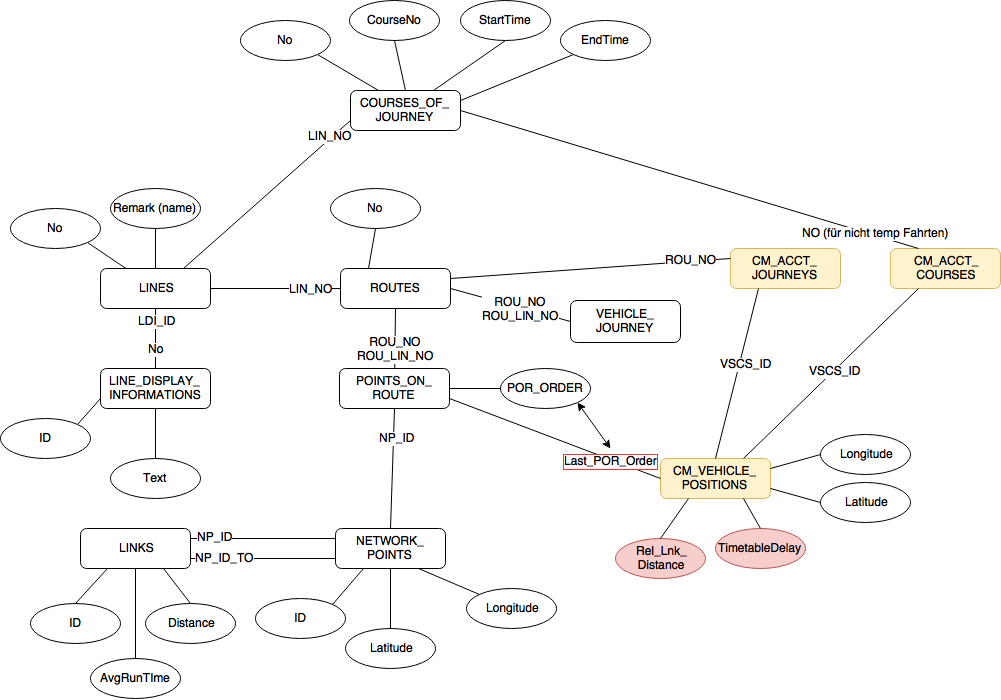
\includegraphics[width=15cm]{res/BVG-DB.png}
	\caption{Datenbank Schema aus SC05 und SC51}
	\label{img:db-bvg}
\end{figure}

\subsection{OSM}
Wie kommt man an die Routen Infos zu den Bus-/Tram Linien. GeoJson.

\section{Komponenten}
Bestandteile des Systems beschreiben (Server, App, ...)

\section{Rest API Schnittstellendefinition}
Der Server f�r die Datenverwaltung basiert auf einer Rest API. Im folgenden Abschnitt werden alle m�glichen Requests zu Ressourcen allgemein und mithilfe eines Beispiels echter Daten beschrieben. W�hrend der Projektarbeit besteht die M�glichkeit, die API �ber den Server \url{http://bus.f4.htw-berlin.de:4545} aus dem HTW-Berlin Netz zu nutzen.
% ##########    GET  /api/v1/route/<ref>    ###########
\subsection{Request f�r Routen einer Linie}
Anfrage aller Routen einer Linie (Beispiel Buslinie). Eine Linie hat mehrere Routen.

\subsubsection{HTTP-Method}
GET

\subsubsection{Resource}
/api/v1/route/\textless ref\textgreater

\subsubsection{Parameters}
\begin{itemize}
	\item ref: Liniennummer
\end{itemize}

\subsubsection{Response}
\begin{lstlisting}
[ {
  "id" : <id>,
  "osmId" : "relation/<osmId>",
  "ref" : "<line number>",
  "name" : "<description of the route>",
  "type" : "<transport type>",
  "network" : "<full name of network>",
  "operator" : "<full name of operator>",
  "from" : "<name of start station>",
  "to" : "<name of end station>",
  "routeType" : "<MULTILINE | LINE>"
} ]
\end{lstlisting}

\subsubsection{HTTP status codes}
\begin{itemize}
	\item 200: Request erfolgreich
	\item 404: Keine Routen gefunden
\end{itemize}

\subsubsection{Beispiel Request}
GET \url{http://domain.com/api/v1/route/M11}

\subsubsection{Beispiel Response}
\begin{lstlisting}
[ {
  "id" : 217,
  "osmId" : "relation/2088816",
  "ref" : "M11",
  "name" : "Buslinie M11: S Sch�neweide => U Dahlem Dorf",
  "type" : "bus",
  "network" : "Verkehrsverbund Berlin-Brandenburg",
  "operator" : "Berliner Verkehrsbetriebe",
  "from" : "S Sch�neweide",
  "to" : "U Dahlem Dorf",
  "routeType" : "MULTILINE"
}, {
  "id" : 218,
  "osmId" : "relation/2088817",
  "ref" : "M11",
  "name" : "Buslinie M11: U Dahlem Dorf => S Sch�neweide",
  "type" : "bus",
  "network" : "Verkehrsverbund Berlin-Brandenburg",
  "operator" : "Berliner Verkehrsbetriebe",
  "from" : "U Dahlem Dorf",
  "to" : "S Sch�neweide",
  "routeType" : "MULTILINE"
} ]
\end{lstlisting}


% ##########    GET  /api/v1/route/geo/<ref>    ###########
\subsection{Request f�r GeoJson einer Route mit ID}
Anfrage einer Route per Id. Das Format der Response ist GeoJson Format.

\subsubsection{HTTP-Method}
GET

\subsubsection{Resource}
/api/v1/route/geo/\textless id\textgreater

\subsubsection{Parameters}
\begin{itemize}
	\item id: Route ID
\end{itemize}

\subsubsection{Response}
\begin{lstlisting}
{
  "type": "Feature",
  "properties": {
    "ref": "<id>",
    "name": "<description of the route>",
    "@id": "relation/<osmId>"
    "from": "<name of start station>",
    "to": "<name of end station>",
    "type": "<transport type>",
    "operator": "<full name of operator>",
    "network": "<full name of network>"
  },
  "geometry": {
    "type": "<MultiLineString | LineString>",
    "coordinates":[]
  }
}
\end{lstlisting}

\subsubsection{HTTP status codes}
\begin{itemize}
	\item 200: Request erfolgreich
	\item 400: Ung�ltiger Parameter
	\item 404: Keine Route gefunden
\end{itemize}

\subsubsection{Beispiel Request}
GET \url{http://domain.com/api/v1/route/geo/67}

\subsubsection{Beispiel Response}
\begin{lstlisting}
{
  "type": "Feature",
  "properties": {
    "ref": "67",
    "name": "Stra�enbahnlinie 67: Krankenhaus K�penick => S Sch�neweide",
    "from": "Krankenhaus K�penick",
    "@id": "relation/2084473",
    "to": "S Sch�neweide",
    "type": "tram",
    "operator": "Berliner Verkehrsbetriebe",
    "network": "Verkehrsverbund Berlin-Brandenburg"
  },
  "geometry": {
    "type": "MultiLineString",
    "coordinates": [
      [
        [
          13.5939995,
          52.4385062
        ],
        [
          13.5939794,
          52.438533
        ], ....
    ]
  }
}
\end{lstlisting}


% ##########    POST  /api/v1/route    ###########
\subsection{Hinzuf�gen einer Route}
F�gt eine Route (oder mehrere) hinzu. Der Payload muss im GeoJson Format sein.

\subsubsection{HTTP-Method}
POST

\subsubsection{Resource}
/api/v1/route

\subsubsection{Payload}
\begin{lstlisting}
{
  "type": "FeatureCollection",
  "features": [
    {
      "type": "Feature",
      "properties": {
        "@id": "relation/<osmId>",
        "name": "<description of the route>",
        "network": "<full name of network>",
        "operator": "<full name of operator>",
        "from": "<name of start station>",
        "to": "<name of end station>",
        "ref": "<id>",
        "route": "<transport type>",
        "type": "route",
      },
      "geometry": {
        "type": "<MultiLineString | LineString>",
        "coordinates": [
        ]
     }
  }
}
\end{lstlisting}

\subsubsection{HTTP status codes}
\begin{itemize}
	\item 201: Resource erstellt
	\item 500: Bad payload
\end{itemize}

\subsubsection{Beispiel Request}
POST \url{http://domain.com/api/v1/route}

\begin{lstlisting}
{
  "type": "Feature",
  "properties": {
    "ref": "67",
    "name": "Stra�enbahnlinie 67: Krankenhaus K�penick => S Sch�neweide",
    "from": "Krankenhaus K�penick",
    "@id": "relation/2084473",
    "to": "S Sch�neweide",
    "type": "tram",
    "operator": "Berliner Verkehrsbetriebe",
    "network": "Verkehrsverbund Berlin-Brandenburg"
  },
  "geometry": {
    "type": "MultiLineString",
    "coordinates": [
       [
         [
         13.5939995,
         52.4385062
       ],
       [
         13.5939794,
         52.438533
      ], ....
    ]
  }
}
\end{lstlisting}


% ##########    GET  /api/v1/journey    ###########
\subsection{Request f�r eine Journey}
Anfrage f�r Messwerte einer Fahrt (Journey) auf einer Route. Die Antwort enth�lt die bereits gegl�tteten Koordinaten.

\subsubsection{HTTP-Method}
GET

\subsubsection{Resource}
/api/v1/journey/\textless id\textgreater

\subsubsection{Parameters}
\begin{itemize}
	\item id: Journey ID
\end{itemize}

\subsubsection{Response}
\begin{lstlisting}
{
  "id": <journeyId>,
  "routeId": <routeId>,
  "startTime": <timeStamp>,
  "endTime": <timeStamp>,
  "points": [
    {
      "id": <id>,
      "journeyId": <journeyId>,
      "time": <timeStamp>,
      "lngLat": {
        "lng": <longitude>,
        "lat": <latidute>
      }
    }, ...
  ]
}
\end{lstlisting}

\subsubsection{HTTP status codes}
\begin{itemize}
	\item 200: Anfrage erfolgreich
	\item 400: Ung�ltiger Parameter
	\item 404: Keine Journey gefunden
\end{itemize}

\subsubsection{Beispiel Request}
GET \url{http://domain.com/api/v1/journey/2}

\subsubsection{Beispiel Response}
\begin{lstlisting}
{
  "id": 2,
  "routeId": 67,
  "startTime": 1513596120000,
  "endTime": 1513597500000,
  "points": [
    {
      "id": 93,
      "journeyId": 2,
      "time": 1513596185100,
      "lngLat": {
        "lng": 13.5916396,
        "lat": 52.4390415
      }
    }, ...
  ]
}
\end{lstlisting}


% ##########    POST  /api/v1/journey    ###########
\subsection{Hinzuf�gen einer neuen Journey}
Erstellt eine neue Journey.

\subsubsection{HTTP-Method}
POST

\subsubsection{Resource}
/api/v1/journery

\subsubsection{Payload}
\begin{lstlisting}
{
  "routeId" : <routeId>,
  "startTime": <timestamp>,
  "endTime": <timestamp>
}
\end{lstlisting}


\subsubsection{Response}
\begin{lstlisting}
<id>
\end{lstlisting}

\subsubsection{HTTP status codes}
\begin{itemize}
	\item 201: Resource erstellt
	\item 400: Bad payload
\end{itemize}

\subsubsection{Beispiel Request}
POST \url{http://domain.com/api/v1/journey}

\begin{lstlisting}
{
  "routeId" : 67,
  "startTime": 1513596120000,
  "endTime": 1513597500000
}
\end{lstlisting}

\subsubsection{Beispiel Response}
\begin{lstlisting}
7
\end{lstlisting}


% ##########    POST  /api/v1/journey/position    ###########
\subsection{Hinzuf�gen einer Messposition f�r die Zeitmessung}
F�gt einen neuen Messpunkt f�r eine Route einer Journey hinzu. Eine Journey beschreibt eine konkrete Fahrt auf einer konkreten Route.

\subsubsection{HTTP-Method}
POST

\subsubsection{Resource}
/api/v1/journey/position

\subsubsection{Payload}
\begin{lstlisting}
{
  "journeyId" : <journeyId>,
  "time": <timestamp>,
  "lngLat" : {
    "lng": <longitude>,
    "lat": <latitude>
  }
}
\end{lstlisting}


\subsubsection{Response}
\begin{lstlisting}
<id>
\end{lstlisting}

\subsubsection{HTTP status codes}
\begin{itemize}
	\item 201: Resource erstellt
	\item 400: Bad payload
\end{itemize}

\subsubsection{Beispiel Request}
POST \url{http://domain.com/api/v1/journey/position}

\begin{lstlisting}
{
  "time":1467888902,
  "journeyId": 3,
  "lngLat": {
    "lat":13.43546,
    "lng":52.32332	
  }
}
\end{lstlisting}

\subsubsection{Beispiel Response}
\begin{lstlisting}
251
\end{lstlisting}


% ##########    GET  /api/v1/vehicle    ###########
\subsection{Request f�r ein Fahrzeug}
Anfrage f�r ein Fahrzeug. Die Antwort enth�lt Geo Daten und Routeninformationen.

\subsubsection{HTTP-Method}
GET

\subsubsection{Resource}
/api/v1/vehicle/\textless id\textgreater

\subsubsection{Parameters}
\begin{itemize}
	\item id: Unique Id des Fahrzeuges (Devices)
\end{itemize}

\subsubsection{Response}
\begin{lstlisting}
{
  "id": <id>,
  "ref": "<uniqueId>",
  "routeId": <routeId>,
  "time": <timeStamp>,
  "position": {
    "lng": <longitude>,
    "lat": <latitude>
  },
  "pastedDistance" : <meter>
}
\end{lstlisting}

\subsubsection{HTTP status codes}
\begin{itemize}
	\item 200: Anfrage erfolgreich
	\item 404: Kein Fahrzeug gefunden
\end{itemize}

\subsubsection{Beispiel Request}
GET \url{http://domain.com/api/v1/journey/2}

\subsubsection{Beispiel Response}
\begin{lstlisting}
{
  "id": 1,
  "ref": "636c81cc2361acd7",
  "routeId": 67,
  "time": 1513596185100,
  "position": {
    "lng": 52.3453,
    "lat": 13.53234
  },
  "pastedDistance" : 5592.54969445254
}
\end{lstlisting}


% ##########    POST  /api/v1/vehicle    ###########
\subsection{Hinzuf�gen eines Fahrzeuges}
F�gt ein neues Fahrzeug der Datenbank hinzu.

\subsubsection{HTTP-Method}
POST

\subsubsection{Resource}
/api/v1/vehicle

\subsubsection{Payload}
\begin{lstlisting}
{
  "ref": "<uniqueId>",
  "routeId": <routeId>,
  "time": <timeStamp>,
  "position": {
    "lng": <longitude>,
    "lat": <latitude>
  }
}
\end{lstlisting}


\subsubsection{Response}
\begin{lstlisting}
<id>
\end{lstlisting}

\subsubsection{HTTP status codes}
\begin{itemize}
	\item 201: Resource erstellt
	\item 400: Bad payload
\end{itemize}

\subsubsection{Beispiel Request}
POST \url{http://domain.com/api/v1/vehicle}

\begin{lstlisting}
{
  "ref": "636c81cc2361acd7",
  "routeId": 67,
  "time": 1513596185100,
  "position": {
    "lng": 52.3453,
    "lat": 13.53234
  }
}
\end{lstlisting}

\subsubsection{Beispiel Response}
\begin{lstlisting}
2
\end{lstlisting}


% ##########    PUT  /api/v1/vehicle    ###########
\subsection{Update eines Fahrzeuges} \label{sub:vehicle:put}
Aktualisiert die Daten eines Fahrzeuges in der Datenbank.

\subsubsection{HTTP-Method}
PUT

\subsubsection{Resource}
/api/v1/vehicle/\textless id\textgreater

\subsubsection{Payload}
\begin{lstlisting}
{
  "ref": "<uniqueId>",
  "routeId": <routeId>,
  "time": <timeStamp>,
  "position": {
    "lng": <longitude>,
    "lat": <latitude>
  }
}
\end{lstlisting}

\subsubsection{HTTP status codes}
\begin{itemize}
	\item 201: Resource erstellt
	\item 400: Bad payload
\end{itemize}

\subsubsection{Beispiel Request}
PUT \url{http://domain.com/api/v1/vehicle/636c81cc2361acd7}

\begin{lstlisting}
{
  "ref": "636c81cc2361acd7",
  "routeId": 67,
  "time": 1513596185100,
  "position": {
    "lng": 52.3453,
    "lat": 13.53234
  }
}
\end{lstlisting}


% ##########    GET  /api/v1/vehicle/id/list    ###########
\subsection{Request f�r ein Fahrzeug} \label{sub:vehicle:list}
Anfrage aller Fahrzeuge, die mit einem Fahrzeug in Verbindung stehen. Das bedeutet, die Antwort enth�lt alle Fahrzeuge auf der Route des angefragten Fahrzeuges.

\subsubsection{HTTP-Method}
GET

\subsubsection{Resource}
/api/v1/vehicle/\textless id\textgreater/list

\subsubsection{Parameters}
\begin{itemize}
	\item id: Unique Id des Fahrzeuges (Devices)
\end{itemize}

\subsubsection{Response}
\begin{lstlisting}
[ {
  "ref" : "<devideId>",
  "geoLngLat" : {
    "lng" : <longitude>,
    "lat" : <latitude>
  },
  "relativeDistance" : <distanceMetersToRequestedVehicle>,
  "relativeTimeDistance": <distanceMilliSecondsToRequestedVehicle>
} ]
\end{lstlisting}

\subsubsection{HTTP status codes}
\begin{itemize}
	\item 200: Anfrage erfolgreich
	\item 404: Kein Fahrzeug gefunden
\end{itemize}

\subsubsection{Beispiel Request}
GET \url{http://domain.com/api/v1/vehicle/636c81cc2361acd7/list}

\subsubsection{Beispiel Response}
\begin{lstlisting}
[ {
  "ref" : "636c81cc2361acd7",
  "geoLngLat" : {
    "lng" : 13.5395005,
    "lat" : 52.4575977
  },
  "relativeDistance" : 0.0
}, {
  "ref" : "4dcghc4zzc6cghcf",
  "geoLngLat" : {
    "lng" : 13.5716218,
    "lat" : 52.4511964
  },
  "relativeDistance" : 2504.827656693912,
  "relativeTimeDistance": 411008
} ]
\end{lstlisting}

% ##########    GET  /api/v1/vehicles    ###########
\subsection{Request f�r die historischen Daten aller Fahrzeuge} \label{sub:vehicle:list}
Anfrage aller historischen Fahrzeugdaten.

\subsubsection{HTTP-Method}
GET

\subsubsection{Resource}
/api/v1/vehicles

\subsubsection{Response}
\begin{lstlisting}
[ {
  "ref": "<uniqueId>",
  "routeId": <routeId>,
  "time": <timeStamp>,
  "position": {
    "lng": <longitude>,
    "lat": <latitude>
  }
} ]
\end{lstlisting}

\subsubsection{HTTP status codes}
\begin{itemize}
	\item 200: Anfrage erfolgreich
	\item 404: Kein Fahrzeug gefunden
\end{itemize}

\subsubsection{Beispiel Request}
GET \url{http://domain.com/api/v1/vehicles}

\subsubsection{Beispiel Response}
\begin{lstlisting}
[ {
  "ref": "636c81cc2361acd7",
  "routeId": 67,
  "time": 1513596185100,
  "position": {
    "lng": 52.3453,
    "lat": 13.53234
  }
} ]
\end{lstlisting}


% ##########    GET  /api/v1/vehicles/id    ###########
\subsection{Request f�r die historischen Daten eines Fahrzeugs} \label{sub:vehicle:list}
Anfrage aller historischen Fahrzeugdaten.

\subsubsection{HTTP-Method}
GET

\subsubsection{Resource}
/api/v1/vehicles/\textless id\textgreater


\subsubsection{Parameters}
\begin{itemize}
	\item id: Unique Id des Fahrzeuges (Devices)
\end{itemize}


\subsubsection{Response}
\begin{lstlisting}
[ {
  "ref": "<uniqueId>",
  "routeId": <routeId>,
  "time": <timeStamp>,
  "position": {
    "lng": <longitude>,
    "lat": <latitude>
  }
} ]
\end{lstlisting}

\subsubsection{HTTP status codes}
\begin{itemize}
	\item 200: Anfrage erfolgreich
	\item 404: Kein Fahrzeug gefunden
\end{itemize}

\subsubsection{Beispiel Request}
GET \url{http://domain.com/api/v1/vehicles/636c81cc2361acd7}

\subsubsection{Beispiel Response}
\begin{lstlisting}
[ {
  "ref": "636c81cc2361acd7",
  "routeId": 67,
  "time": 1513596185100,
  "position": {
    "lng": 52.3453,
    "lat": 13.53234
  }
} ]
\end{lstlisting}


\section{Datenbankschema Server}